\thispagestyle{empty}
\chapter{Análisis de Semejantes}

Tal y como se ha reflejado en la introducción, el proceso a seguir para optener un diseño preliminar, será el análisis de semejantes.
Este análisis consiste en crear una base de datos de aeronaves ya existentes, cuyas características sean similares a las que podría tener la nuestra, de manera que mediante un análisis estadístico se pueda obtener una primera aproximación de algunas características de nuestra aeronave.\\

Dado que el objetivo es el diseño de un helicóptero no tripulado de 450 Kg de \emph{MTOW}, los vehículos a analizar serán helicópteros de una masa similar, en torno a 400-500 kg, pero al no existir una cantidad suficiente dentro de este margen, se ha decidido ampliar este.
En la siguiente tabla se encuentran los helicópteros seleccionados para el análisis

%PROBLEMAS CON LAS TABLAS, BUSCAR COMO ARREGLAR EL DESASTRE DE TABLA QUE NO ENTRA, TAL VEZ DIVIDIRLO EN 2 SEA SUFICIENTE

Como se observa, parte de la tabla se encuentra en blanco. Estos datos no han sido facilitados por los fabricantes y por ello no salen reflejados.
Tambien se observa que se hace distinción entre \emph{UAVs} y vehículos tripulados, como dato meramente curioso que refleja que en el margen de pesos elegido, es dificil encontrar aeronaves tripuladas.\\

Una vez se ha obtenido la selección de aeronaves semejantes, se procede a realizar un análisis estadístico de las distintas características de los mismos para obtener unos primeros valores de diseño. Al ser la característica más definitoria de la aeronave el peso máximo al despegue, se observará la evolución de los distintos parámetros con el MTOW.
En este capítulo se pueden observar las gráficas que se obtienen del análisis anterior para cada parámetro, incluyendo una línea de tendencia que nos permita obtener una primera aproximación en el diseño. Cabe indicar que se han omitido, en las gráficas correspondientes, aquellos vehículos cuyas características no eran conocidas, sin eliminarlos del resto de ellas. Las líneas de tendencia se han generado usando una aproximación lineal, lo cual puede llevar a una mala aproximación dependiendo de los datos.


\begin{figure}
	\centering
	\includegraphics[width=80mm]{graficos/anald}
	\caption{Relación entre los diámetros de las palas de los helicópteros y sus MTOW junto a su línea de tendencia}
\end{figure}
\begin{figure}
	\centering
	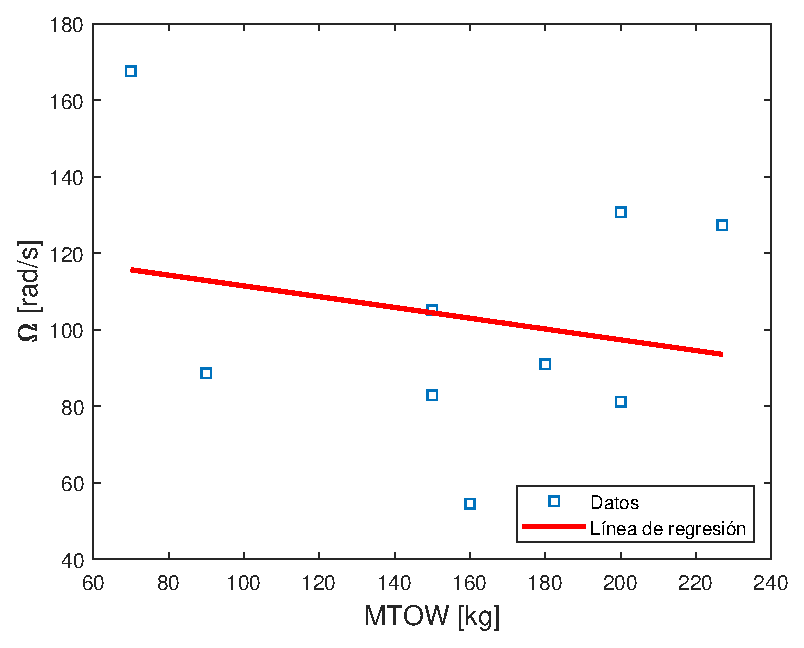
\includegraphics[width=80mm]{graficos/analomega}
	\caption{Relación entre las velocidades de giro del rotor de los helicópteros y sus MTOW junto a su línea de tendencia}
\end{figure}
\begin{figure}
	\centering
	\includegraphics[width=80mm]{graficos/analb}
	\caption{Relación entre el número de palas del rotor principal de los helicópteros y sus MTOW junto a su línea de tendencia}
\end{figure}
\begin{figure}
	\centering
	\includegraphics[width=80mm]{graficos/analbtr}
	\caption{Relación entre el número de palas del rotor antipar de los helicópteros y sus MTOW junto a su línea de tendencia}
\end{figure}
\begin{figure}
	\centering
	\includegraphics[width=80mm]{graficos/analaut}
	\caption{Relación entre las autonomías de los helicópteros y sus MTOW junto a su línea de tendencia}
\end{figure}
\begin{figure}
	\centering
	\includegraphics[width=80mm]{graficos/analtecho}
	\caption{Relación entre los techos de vuelo de los helicópteros y sus MTOW junto a su línea de tendencia}
\end{figure}
%\begin{figure}
%	\centering
%	\includegraphics[width=80mm]{graficos/analalt}
%	\caption{Relación entre las alturas de los helicópteros y sus MTOW junto a su línea de tendencia}
%\end{figure}
\begin{figure}
	\centering
	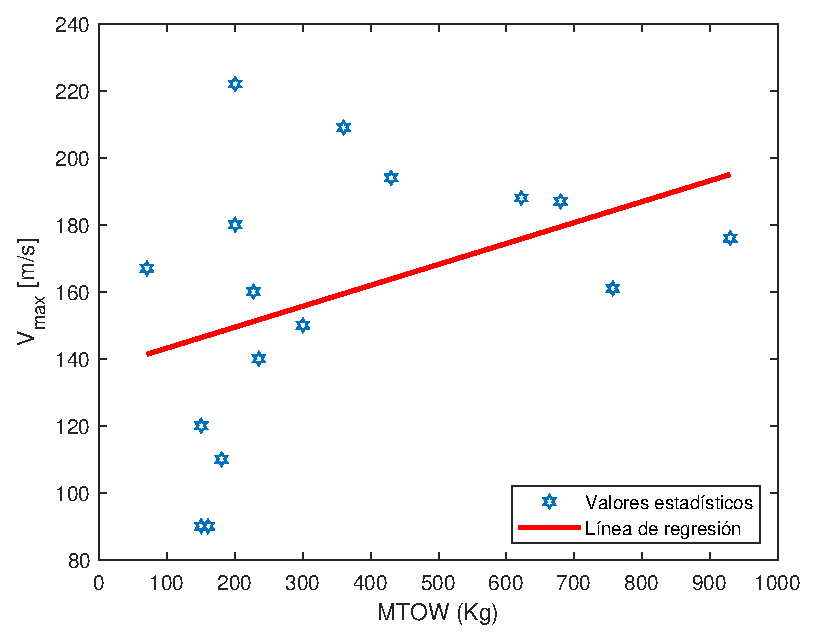
\includegraphics[width=80mm]{graficos/analv}
	\caption{Relación entre las velocidades máximas de avance de los helicópteros y sus MTOW junto a su línea de tendencia}
\end{figure}

Como se puede observar, muchos helicópteros comparten características aunque sus pesos sean muy distintos, y algunas líneas de tendencia se alejan considerablemente de los valores promedio para la zona que corresponde a 450 kg. A la vista de la comparación realizada, se obtienen unos valores iniciales de diseño, a saber:

\begin{itemize}
	\item Diámetro: 5,5 m
	\item Velocidad de giro del rotor: 120 rad/s
	\item Número de palas del rotor principal: 2
	\item Número de palas del rotor antipar: 2
	\item Autonomía: 3 horas
	\item Techo de vuelo: 3200 m
	%\item Altura: 2,4 m
	\item Velocidad de avance máxima: 190 m/s
\end{itemize}

Queda patente que en algunos casos, se han aproximado los valores omitiendo las líneas de tendencia, usando en su lugar los valores de los helicópteros cuyos MTOW son más próximos al de la aeronave a diseñar.